\textbf{Sự Gập và Mở của Protein theo Nhiệt độ}

Ở chương trình giáo khoa THPT, các bạn đã được học về protein trong bộ môn Sinh học lớp 9. Protein là một chuỗi các amino acid được sắp xếp theo thứ tự cụ thể, quyết định cấu trúc và chức năng của protein trong cơ thể. Chuỗi này sau đó sẽ gập lại thành hình dạng ba chiều để thực hiện các chức năng sinh học khác nhau; e.g. protein Chaperone giúp gập cho đúng lại các protein bị gập sai (xem hình \ref{fig:Chaperone}), đảm bảo rằng những protein đó thực hiện được chức năng chính xác. Lưu ý rằng, khi được gập lại đúng cách, protein thường không trở thành một cấu trúc rắn tuyệt đối, mà là một cấu trúc linh động, có thể co duỗi và hoạt động như một ``cỗ máy'' ở kích thước nano. Nói cách khác, khi protein gập đúng cách và hoạt động được, nó không cần nhất thiết phải là \textit{gập hoàn hảo}.

\begin{figure}[!h]
    \centering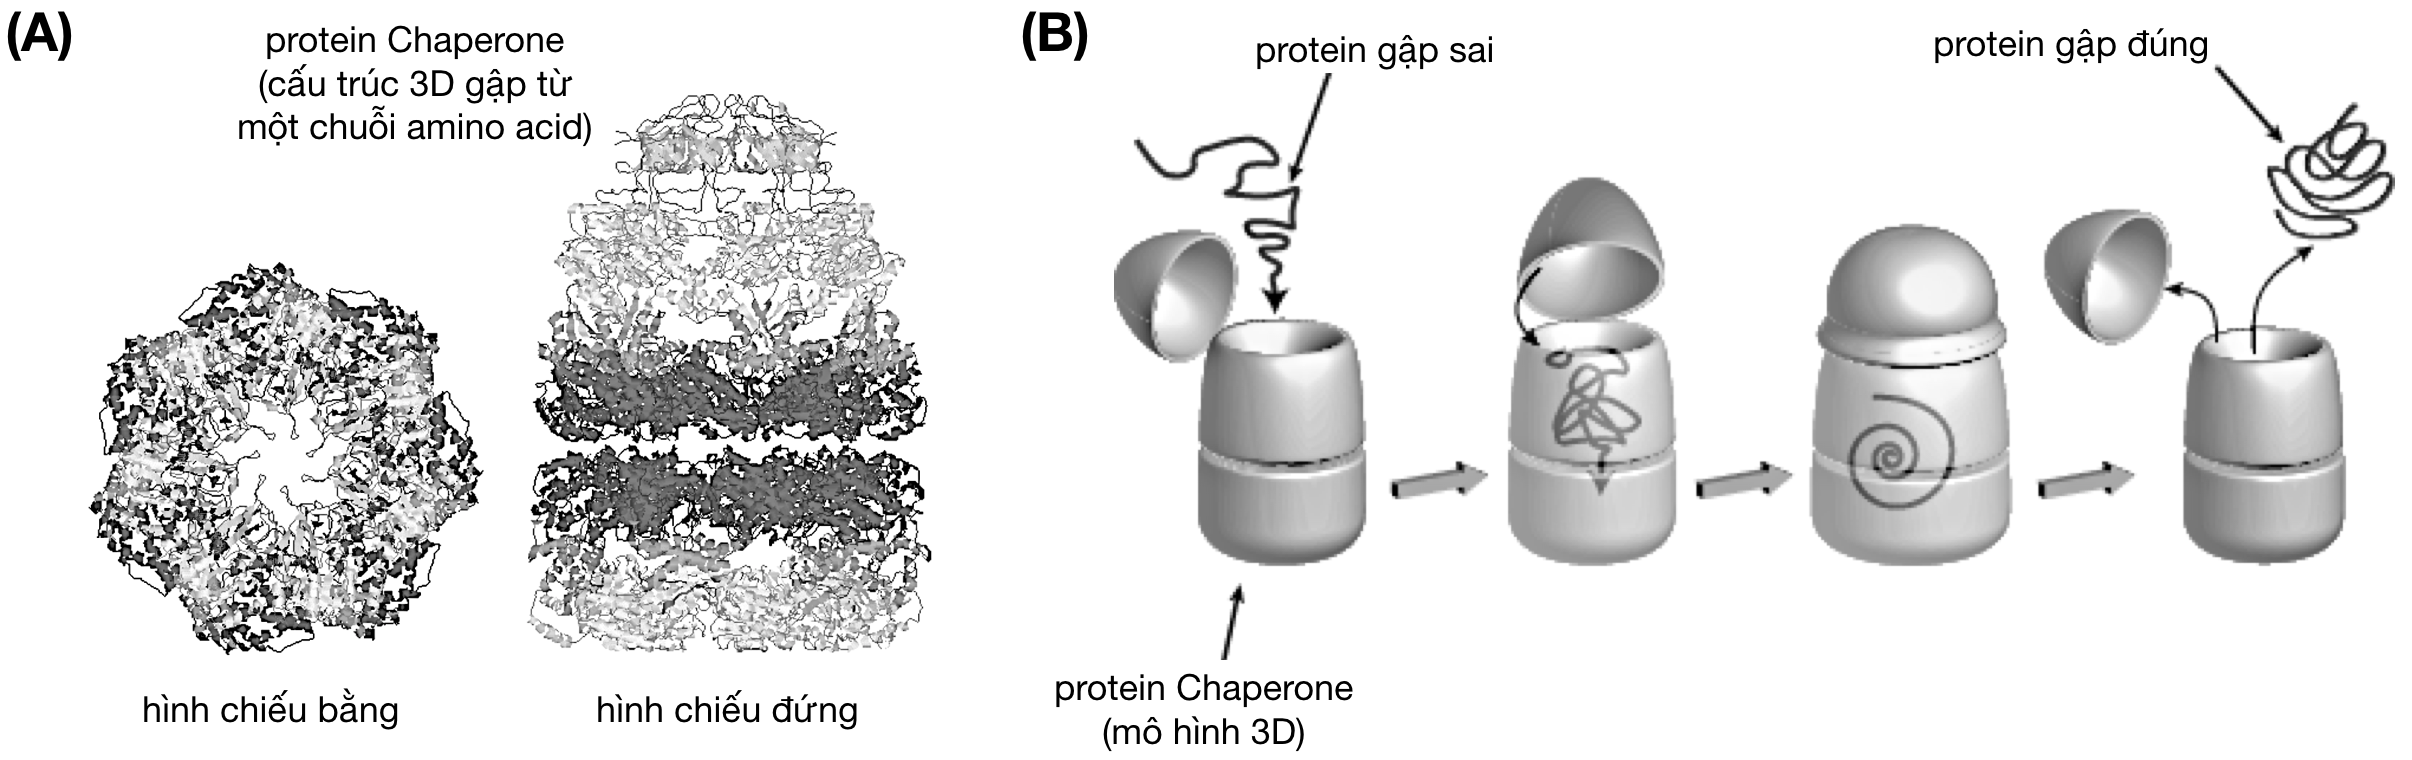
\includegraphics[width=0.96\textwidth]{Problem_2/Figs_P2/fig01.png}\caption{Cấu trúc và chức năng của protein Chaperone. (A) Các hình chiếu của protein Chaperone, mô tả một chuỗi amino acid được gấp lại thành một cấu trúc ba chiều xác định. (B) Các protein bị gấp sai có thể di chuyển vào khoang trung tâm của protein Chaperone, nơi chúng được điều chỉnh và gấp lại đúng cách.}
    \label{fig:Chaperone}
\end{figure}

Tìm hiểu về cấu trúc gập của các loại protein khác nhau là một trong những vấn đề quan trọng nhất trong lĩnh vực Vật lý Sinh học phân tử, và nghiên cứu ứng dụng trí tuệ nhân tạo để giải quyết vấn đề này đã dẫn tới giải Nobel Hóa học năm 2024.

\ \ 

Chúng ta sẽ cùng nhau khám phá sự chuyển trạng thái của protein theo nhiệt độ, từ cấu trúc gập (có khả năng thực hiện chức năng sinh học) sang cấu trúc mở (không còn hoạt động). Cụ thể hơn, chúng ta tìm hiểu về \textit{mô hình khóa kéo}, tuy rất đơn giản, nhưng đủ để mô tả các tương tác giữa những thành phần cấu tạo protein (các amino acid) với môi trường xung quanh (các phân tử nước) ở bậc vi mô, cũng như các tính chất nhiệt động lực học của của đa số các loại protein khác nhau ở bậc vĩ mô.

\ \ 

Trong \textit{mô hình khóa kéo} của protein, mỗi amino acid tại vị trí $j$ được biểu diễn bằng một tham số bit nhị phân $\phi_j \in \{ 0,1 \}$: $\phi_j = 1$ khi amino acid ở đúng vị trí so với trạng thái \textit{gập hoàn hảo}, và $\phi_j = 0$ nếu không đúng. Khi các amino acid từ thứ tự $1$ đến $j$ không ở vị trí \textit{gập hoàn hảo}, amino acid thứ $j$ có thể tương tác với các phân tử nước bên ngoài (đây chính là tính chất \textit{khóa kéo} đặc trưng của mô hình này), được mô tả qua tham số $w_j \in \{ 0,1,2,...,(g-1)\}$, trong đó $g$ là số mức năng lượng tương tác khả dĩ. Với protein gồm $N$ amino acid, chỉ số $j$ sẽ chạy từ $1$ đến $N$. Mỗi \textit{vi thái} $\alpha$ của protein được xác định bởi $2N$ các giá trị tham số:
$$\alpha \equiv \left[ (\phi_1,w_1), (\phi_2,w_2), (\phi_3,w_3), ..., (\phi_N,w_N) \right] \ . $$
Năng lượng của protein khi nó ở \textit{vi thái} $\alpha$ được xác định bởi:
\begin{equation}
\begin{split}
    E_\alpha = & \sum^N_{j=1} \left[-E_0 \prod^j_{k=1} \phi_k + \left(1-\prod^j_{k=1} \phi_k \right)(\mu+w_j \delta ) \right]
    \\
    = &-E_0 \left(\phi_1 + \phi_1 
 \phi_2  + \phi_1 \phi_2 \phi_3 + ... + \phi_1 \phi_2 \phi_3 ... \phi_N \right)
 \\
 &+\Big[(1-\phi_1)(\mu + w_1 \delta ) + (1-\phi_1\phi_2)(\mu + w_2 \delta ) + (1-\phi_1\phi_2 \phi_3)(\mu + w_3 \delta ) 
 \\
 & \ \ \ \ \ \ \ \ + ... + (1-\phi_1\phi_2 \phi_3 ... \phi_N)(\mu + w_N \delta ) \Big] \ ,
\end{split}
\end{equation}
với $E_0>0$, $\mu<0$, và $\delta>0$ là các giá trị mang thứ nguyên năng lượng. 

\ \ 

Khi protein ở nhiệt độ $T$, xác suất $p_\alpha$ nó đang ở \textit{vi thái} $\alpha$ sẽ tuân theo phân bố Maxwell-Boltzmann:
\begin{equation}
    p_\alpha \propto \exp\left( -\frac{E_\alpha}{k_B T} \right) \ ,
\label{prob}
\end{equation}
với $\propto$ là ký hiệu biểu thị mối liên hệ tỉ lệ và $k_B$ là giá trị hằng số Boltzmann. Định nghĩa giá trị nhiệt độ $T_0 \equiv E_0/k_B$. Năng lượng trung bình thống kê $\langle E(T) \rangle$ của protein ở nhiệt độ $T$ được xác định theo giá trị trung bình của năng lượng trên tất cả các \textit{vĩ thái} khả dĩ:
\begin{equation}
    \langle E(T) \rangle = \sum_\alpha p_\alpha E_\alpha
\label{E_avg}
\end{equation}
Nhiệt dung riêng $C_1(T)$ ở nhiệt độ T trên mỗi amino acid của protein được xác định theo phép tính đạo hàm sau đây:
\begin{equation}
    C_1(T) = \frac{d}{dT} \left[\frac{\langle E(T)\rangle}{N} \right] \ .
\label{heat_cap}
\end{equation}
Xét một protein được cấu tạo từ rất rất nhiều amino acid (tức xét giới hạn $N\rightarrow \infty$). Sử dụng các giá trị số sau đây: $\mu/E_0=-2$, $\delta/E_0=0.1$, $g=60$.

\ \ 

\textbf{Câu hỏi a.} Khảo sát giá trị $C_1(T)$ theo đơn vị $k_B$ tại các giá trị nhiệt độ $T$ thỏa mãn:
$$T/T_0=0.6,0.7,0.8,0.9,1.0 \ \  \text{và} \ \   T/T_0=1.4,1.5,1.6,1.7,1.8 \ . $$

\ \  

\textbf{Câu hỏi b.} Chứng minh rằng $C_1(T)$ sẽ phải thay đổi đột ngột tại một số giá trị nhiệt độ. 

\ \ 

Cho biết rằng những giá trị nhiệt độ này tương ứng với sự chuyển pha của protein, từ trạng thái mở sang trạng thái gấp khi $C_1(T)$ nhảy xuống cùng với sự tăng của nhiệt độ $T$, và từ trạng thái gấp sang trạng thái mở khi $C_1(T)$ nhảy lên với sự tăng của $T$. Cũng cho biết chỉ tồn tại duy nhất hai giá trị nhiệt độ chuyển pha.

\ \ 

\textbf{Câu hỏi c.} Hãy ước tính những vùng giá trị tỉ số $T/T_0$ mà protein sẽ ở trạng thái gấp.